\section{Simple Multiplication May Be All You Need}
\label{sec:method} 

\begin{figure}[!t]
%        \hspace{-1mm}
        \begin{minipage}{1\linewidth}
        \centering
        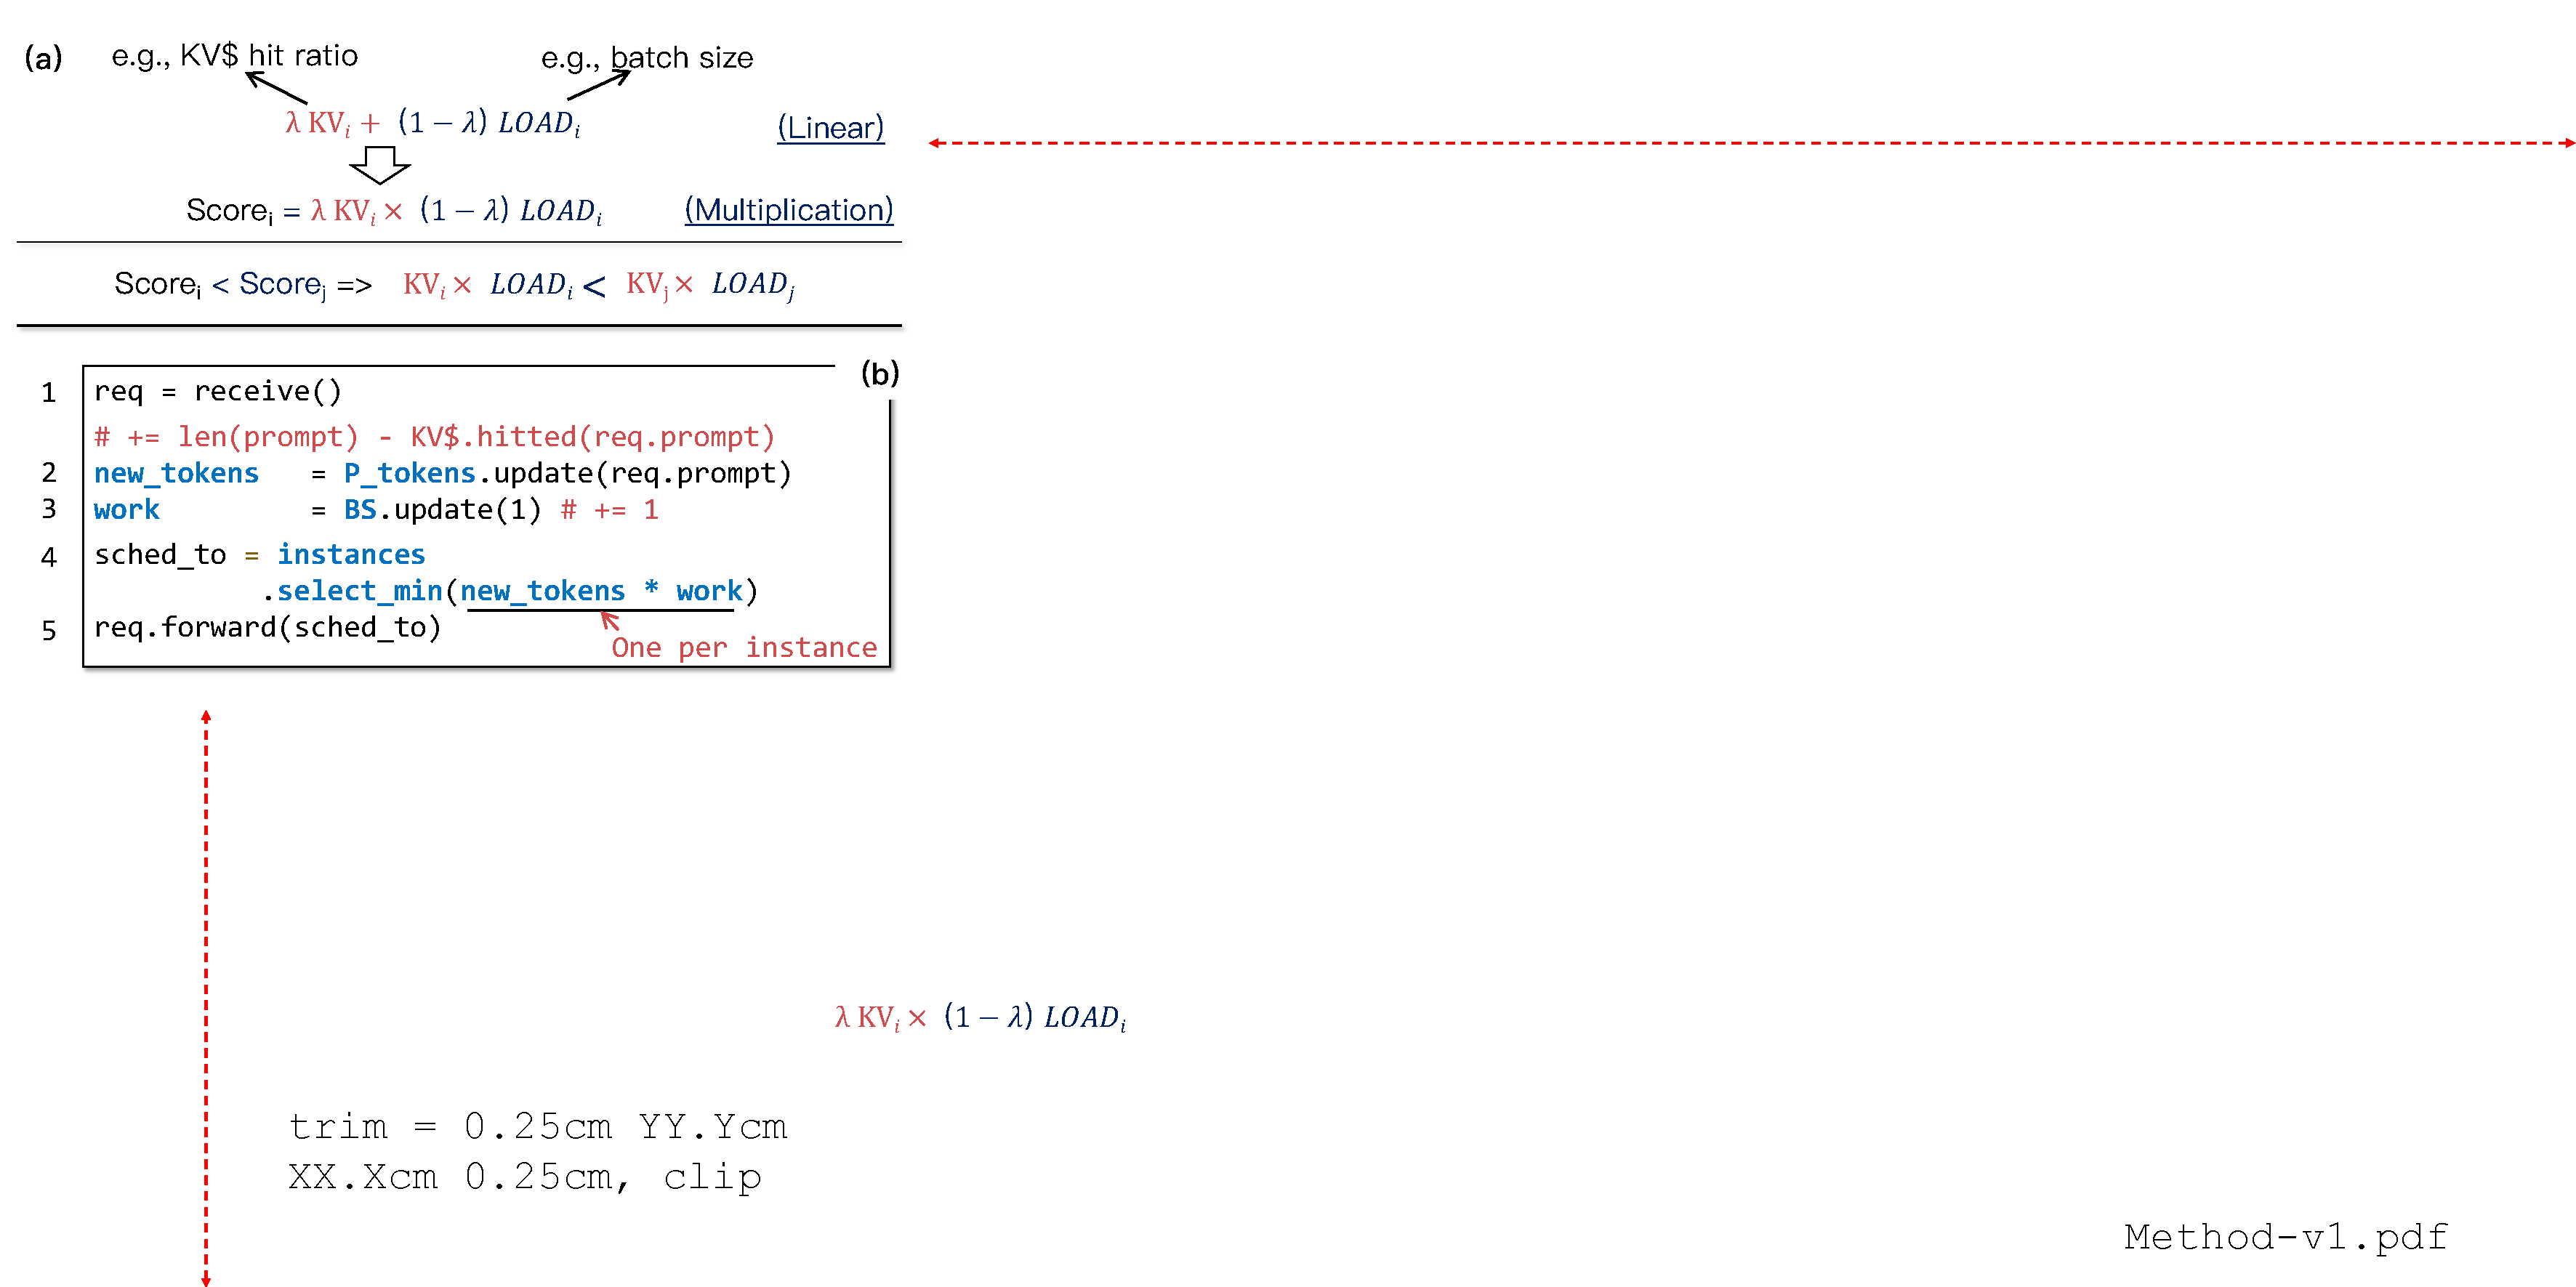
\includegraphics[width=0.95\linewidth, trim=0.25cm 13.5cm 38.4cm 0.25cm, clip]{figs/method-v1.pdf}
        \end{minipage} \\[-1pt]
        \begin{minipage}{1\linewidth}
        \caption{\small{%
    (a) An illustration of how multiplication avoids hyperparameters in combining two indicators
    as would be needed in linear combination, 
    and (b) the pseudocode of our scheduling method.
        }}  
        \label{fig:method}
        \end{minipage} \\[-0pt]
        \end{figure}

\nospacestitle{The methodology ({\fig{fig:method}}). \,}
Our method is simple: we only need to multiply two carefully chosen indicators to compute the scheduling score,
one for {\kvcache}-awareness and the other for load balancing,
and then route the request to the instance with the minimal score.
The basic idea is based on the observation that,
if a linear combination of two indicators works, then multiplication can also work
in a similar manner, with the benefit of avoiding the need for hyperparameter tuning, 
as shown in (a). 
The choice of the two indicators---\textbf{P-token}---the number of new prefill tokens if the request is routed to an instance
considering {\kvcache} hits,
and \textbf{BS}---the batch size of the instance,
is based on our careful analysis in \textsection{\ref{sec:indicators}}.

To see why routing to the instance with the minimal (P-Tokens $\times$ BS) score considers both objectives well,
consider two instances $i$ and $j$:
if routing the request to instance $i$ results in more {\kvcache} hits than routing it to instance $j$,
then instance $i$ will have a lower \textbf{P-token} value unless there are many queued prefill requests in instance $i$
 (indicating work imbalance).
Meanwhile, the \textbf{BS} captures the decode workload of each instance,
so if instance $i$ has a significantly larger batch size than instance $j$,
the multiplication will likely favor instance $j$ for load balancing. 

We should acknowledge that there do exist cases where multiplication may fail due to
extremely skewed {\kvcache} accesses,
i.e., a set of instances is always chosen due to high {\kvcache} hits (low \textbf{P-token}),
and the increased batch size (\textbf{BS}) on these instances cannot compensate for the low \textbf{P-token} values.
Such cases---as we will analyze in \textsection{\ref{sec:m-analyze}}---are rare in practice
and can be detected (and thus mitigated) beforehand.

\subsection{The Choice of the Indicators}
\label{sec:indicators}


\begin{figure}[!t]
%        \hspace{-1mm}
        \begin{minipage}{1\linewidth}
        \centering
        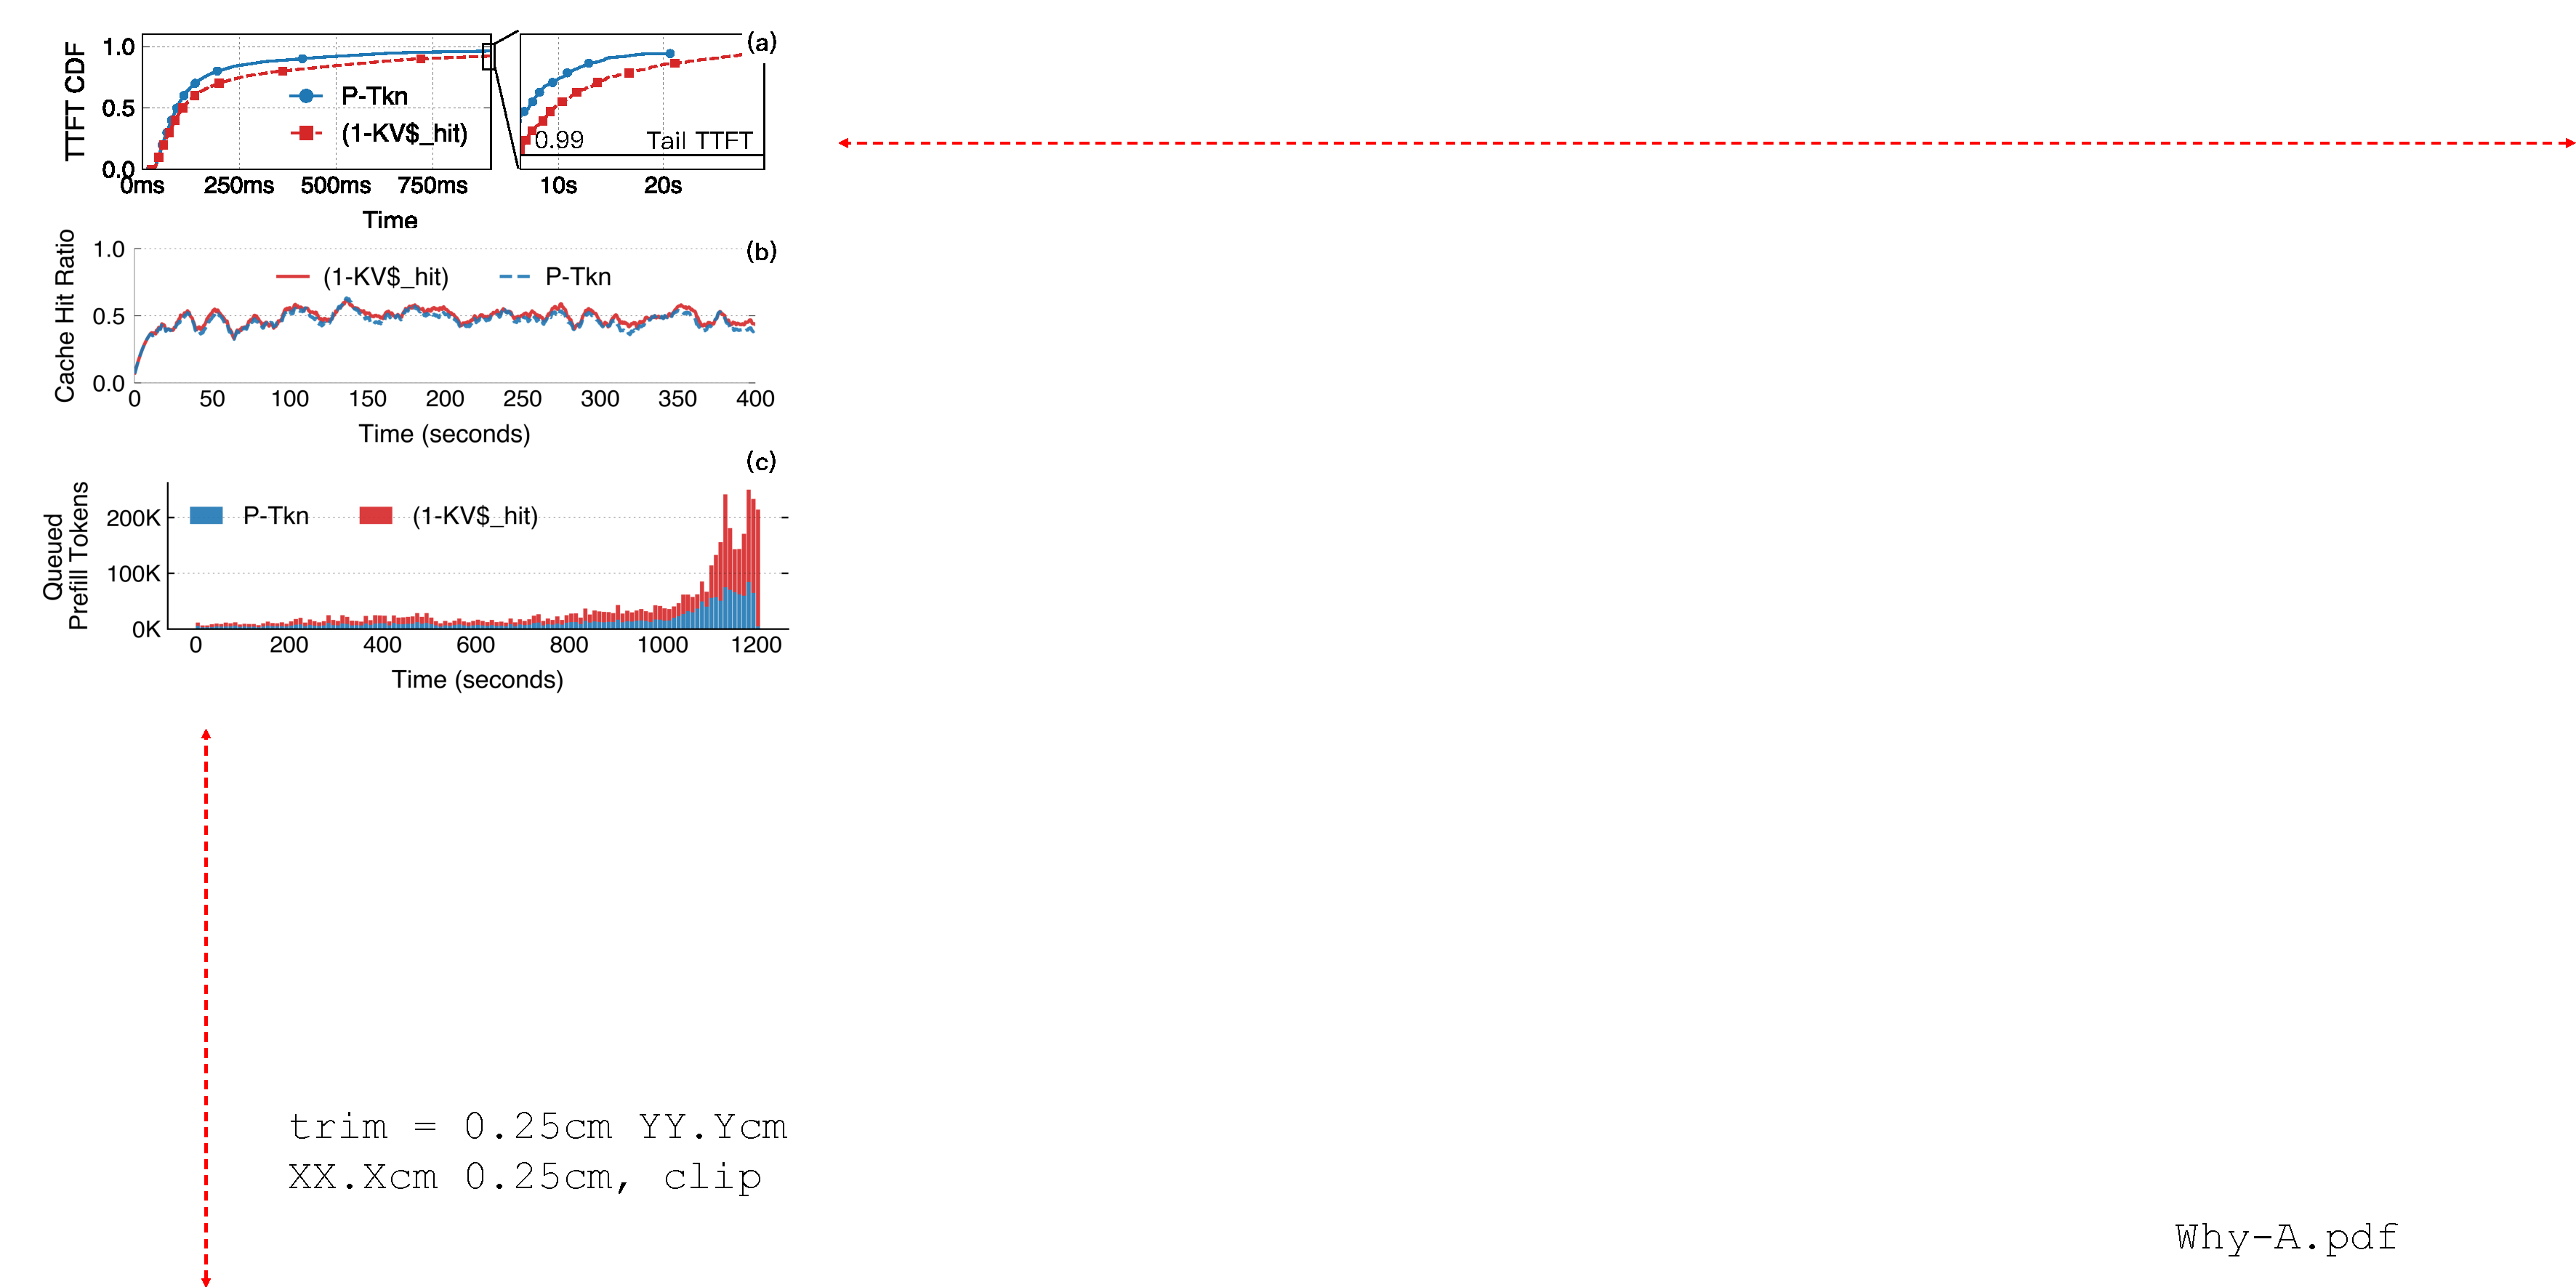
\includegraphics[width=0.99\linewidth, trim=0.25cm 13.1cm 40.5cm 0.25cm, clip]{figs/5-1-select-A-B/why-A.pdf}
        \end{minipage} \\[-1pt]
        \begin{minipage}{1\linewidth}
        \caption{\small{%
    (a) A comparison of using new prefill tokens (P-Tkn) vs. 1-{\kvcache} hit ratio (1-KV$_{hit}$)
    as the {\kvcache}-awareness indicator ($A$) in $A \times BS$ scheduling,
    (b) the {\kvcache} hit ratio analysis, and
    (c) the queued prefill tokens analysis.
    The analysis is done on the Qwen3-30B model with ChatBot(Qwen) trace. 
        }}  
        \label{fig:whyA}
        \end{minipage} \\[-0pt]
        \end{figure}

\nospacestitle{{\kvcache}-awareness indicator (P-token). \,}
Besides \textbf{P-token}, another natural choice for the {\kvcache}-awareness indicator is
the \textbf{1-{\kvcache} hit ratio}, i.e., the {\kvcache} hit ratio if the request is routed to an instance.
It is adopted by works like Preble~\cite{DBLP:conf/iclr/SrivatsaHAL025} and AIGW~\cite{aigw}.
Note that the one minus is because a higher {\kvcache} hit ratio should yield a lower score
to align with the new prefill tokens indicator.
We do not consider TTFT as it requires the development of a simulator,
which is not always applicable.

Our empirical analysis shows that using \textbf{P-token} yields better performance than using \textbf{1-{\kvcache} hit ratio}.
From {\fig{fig:whyA}} (a), it can be observed that using \textbf{P-token} results in a 14.4\% lower
P50 TTFT and a 42.8\% lower P95 TTFT compared to using \textbf{1-{\kvcache} hit ratio}.
For a fair comparison, we fix the load-balancing indicator to \textbf{BS} in both cases.
Note that due to space limitations, we only report the results for one workload here;
however, the trend is consistent across all evaluated workloads.

To understand the cause of this difference,
{\fig{fig:whyA}} further breaks down the {\kvcache} hit ratios of different approaches in (b)
and the load balancing status in (c).
We can see that the two methods achieve similar {\kvcache} hit ratios, so
both approaches are {\kvcache}-aware in a similar manner.
The key difference lies in the fact that using \textbf{P-token} achieves better load balancing,
as it additionally considers the queued prefill tokens in each instance.
As a result, when making scheduling decisions, the router bypasses those instances
containing many queued prefill requests, even if they have a high {\kvcache} hit ratio.


\begin{figure}[!t]
        \hspace{-2mm}
        \begin{minipage}{1\linewidth}
        \centering
        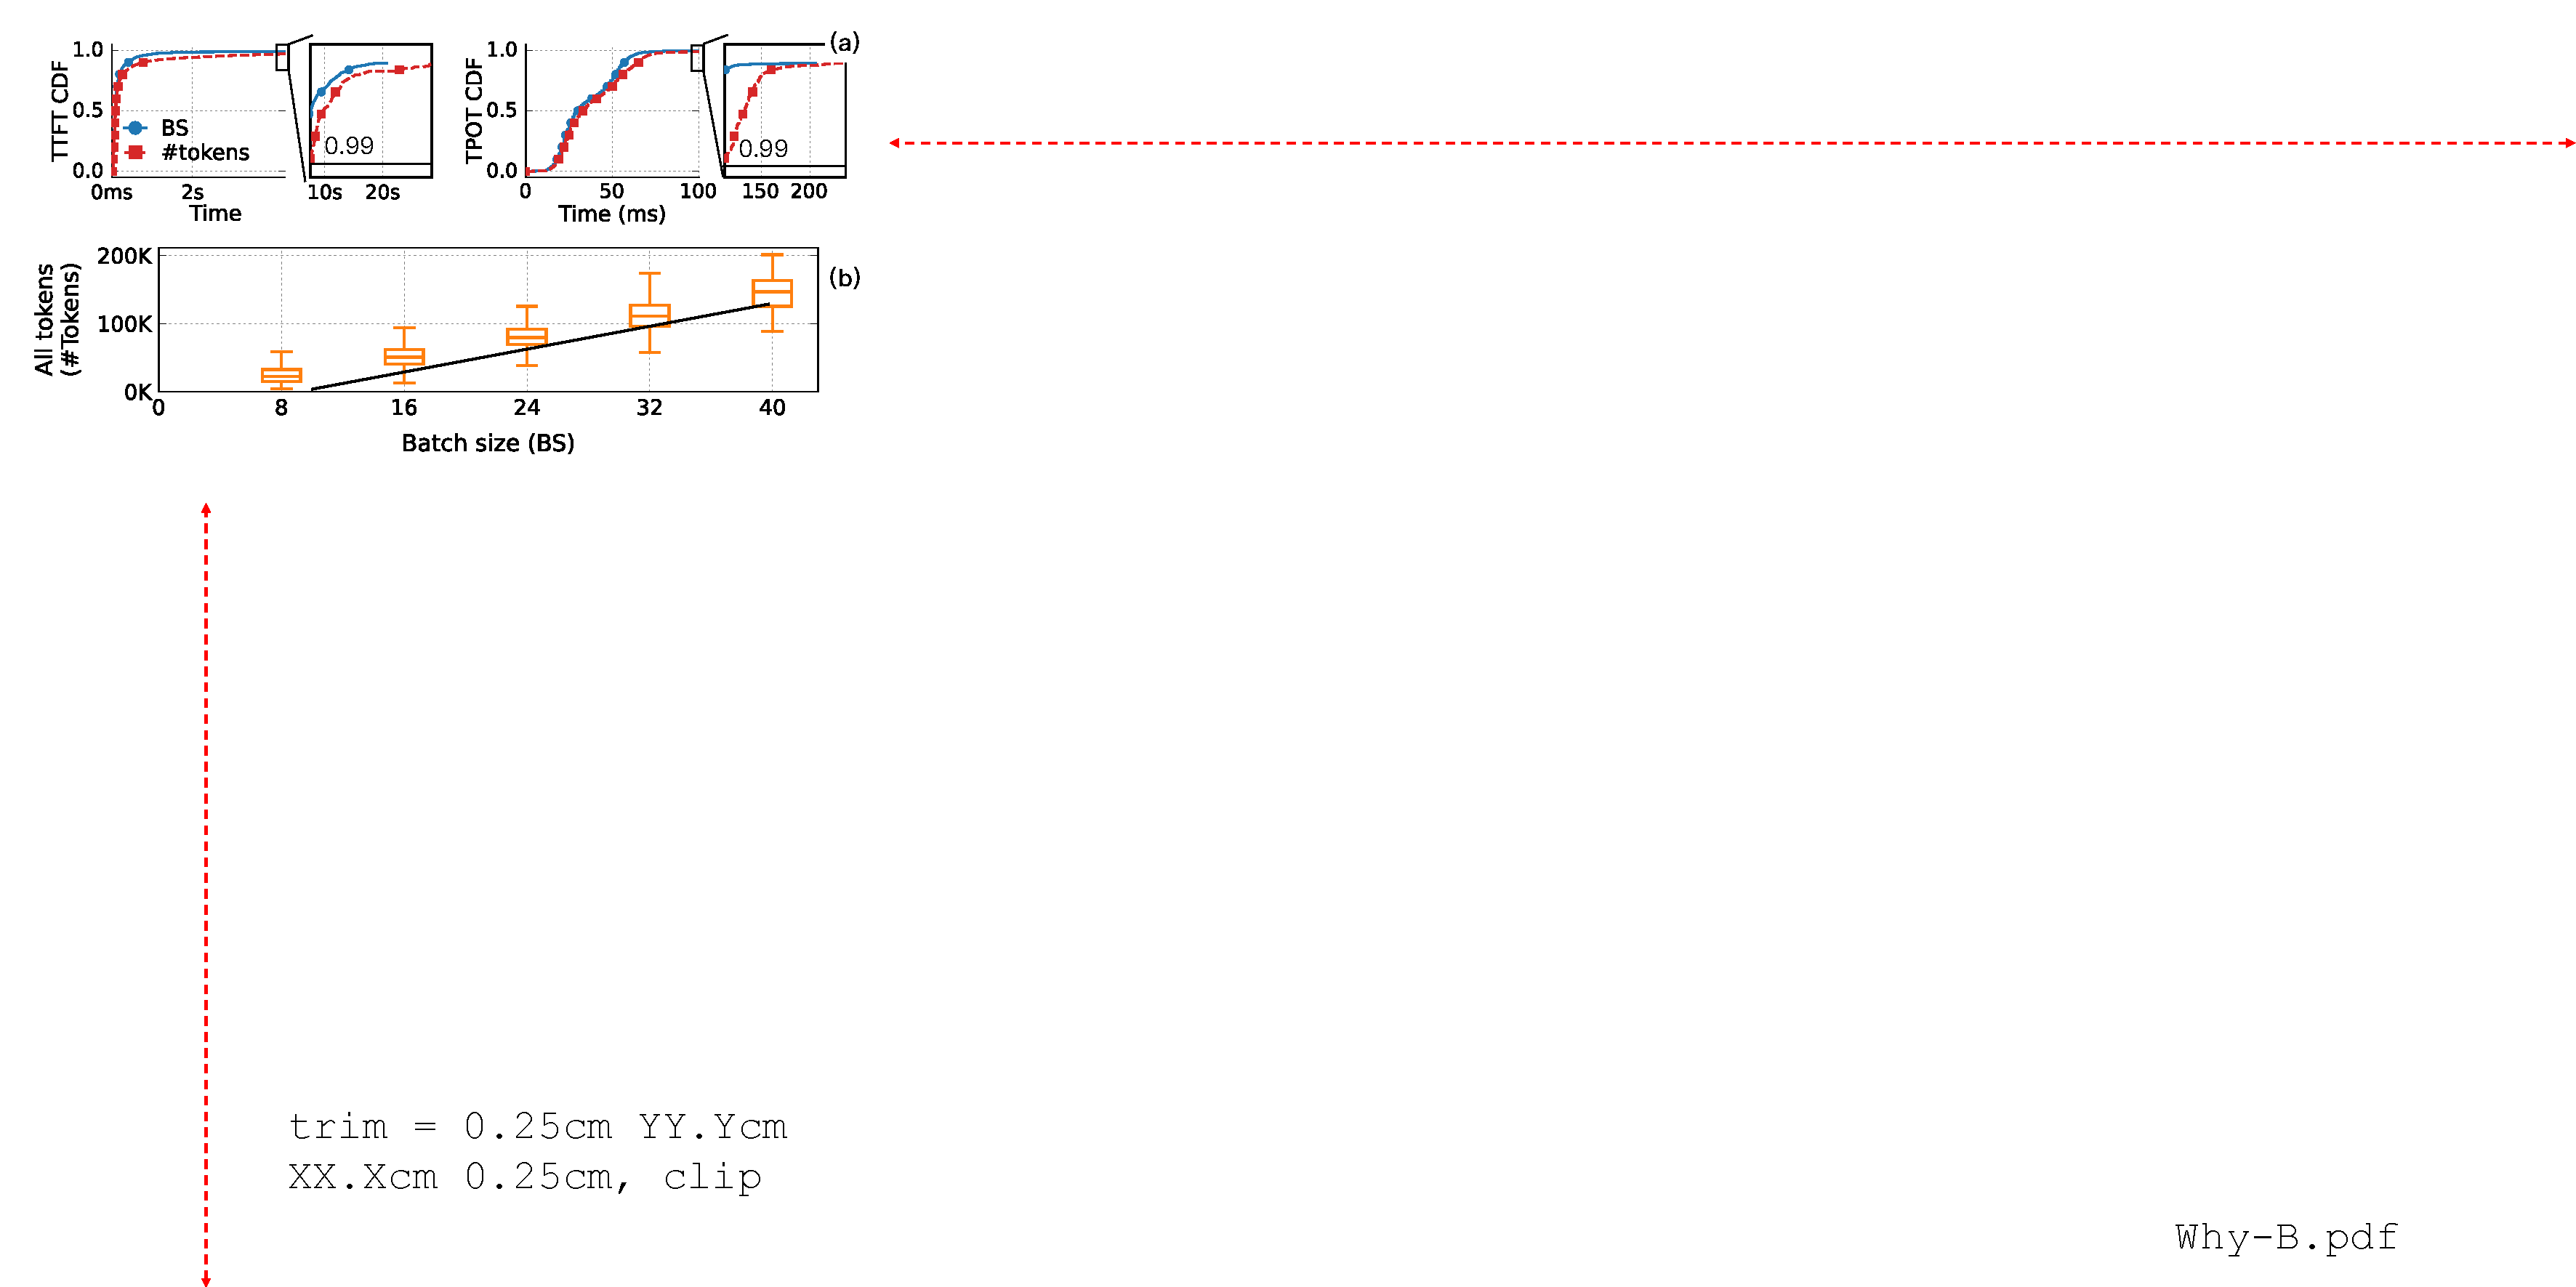
\includegraphics[width=0.99\linewidth, trim=0.25cm 18.5cm 39.5cm 0.25cm, clip]{figs/bs-relation-totaltkns-tbt/why-B.pdf}
        \end{minipage} \\[-2pt]
        \begin{minipage}{1\linewidth}
        \caption{\small{%
    (a) A comparison of using batch size (BS) vs. total tokens (\#Tokens)
    as the load balance indicator ($B$) in $P$-Tokens $\times B$ scheduling. 
    (b) The relationship between batch size and total tokens profiled. 
    The analysis is done on the Qwen3-30B model with ChatBot(Qwen) trace. 
        }}  
        \label{fig:whyB}
        \end{minipage} \\[-0pt]
        \end{figure}


\stitle{Load-balancing indicator (BS). \,}
Besides \textbf{BS}, another common choice is the
total tokens (\textbf{\#Tokens}) on each instance, as adopted by works like ai-Dynamo~\cite{ai-Dynamo}, AIGW~\cite{aigw}.
The rationale is that the total computation cost of a request is proportional
to the number of tokens in its context.
However, we found
using \textbf{BS} yields better performance,
as shown in {\fig{fig:whyB}} (a) due to two reasons.
First, workloads can be categorized into prefill and decode loads,
where the former is considered in our \textbf{P-Tokens} indicator.
Thus, we only need an indicator for the decode workload, which is exactly what \textbf{BS} captures (note that we
have also tried using decode batch size, and the results are similar
since the \textbf{BS} is dominated by the decode requests).
Moreover, \textbf{BS} is a better indicator for the (decode) work assigned to an instance because the decode time
is more stable across different batch sizes,
i.e., a larger batch size leads to a longer decode time,
but a larger decode token may not necessarily lead to a longer decode time
if there is small batch thanks to the {\kvcache}~\cite{DBLP:conf/osdi/ZhongLCHZL0024}.
This is illustrated in {\fig{fig:whyB}} (b),
in which we profile the relationship of the batch size and total tokens  
during serving a ChatBot(Qwen) workload with Qwen3-30B. 


%\subsection{Failure Cases Analysis and Two-phase Detectors for the Failure Cases}
\subsection{Benign and Failure Cases Analysis of Multiplication-based Scheduling Score}
\label{sec:m-analyze}

\nospacestitle{Overview. \,}
At a high level, as long as there is no load imbalance,
i.e., one instance is overloaded while others are idle,
routing requests to instances with high {\kvcache} hit rates (i.e., low \textbf{P-token})
is always beneficial.
Thus, the multiplication fails if a load imbalance is about to occur on a set of instances,
but the increase in \textbf{BS} on these instances cannot offset the decrease in \textbf{P-token} due to high {\kvcache} hit rates
on the about-to-be overloaded instances,
leading requests to be continuously routed to them and causing the imbalance. 
This can happen under extreme {\kvcache} skewness:
when a small set of requests repeatedly accesses the same
prefix on a set of instances---which we term \emph{{\kvcache} hotspots} without considering others.
We found such hotspots are rare in practice---at least not
present in all our evaluated traces and, more
importantly, as their patterns are clear, we can design a detector to catch them beforehand.

Therefore, to analyze the failure cases of our multiplication method,
we need to derive the condition under which {\kvcache} hotspots occur and
the increased batch size cannot offset the high {\kvcache} hit rate given a workload pattern.
For each workload, we first group requests by their {\kvcache} prefixes
and partition instances according to {\kvcache} hit rates.
Afterward, for each request class, we can specifically analyze the
relationship between the workload pattern, the P-token indicator given the {\kvcache} hit rate,
and the batch size indicator.

\stitle{Prelude: request grouping and instance partitioning. \,}
First, we partition all requests into a set of classes
\(\mathcal{C}\), where each \(c\!\in\!\mathcal{C}\) corresponds to a
group of requests that share the same {\kvcache} prefix.
In practice, a class roughly matches an application or a user: their
requests share the same system prompt and often a similar conversation
history~\cite{10.5555/3768039.3768067}.
For a fixed class \(c\), we consider an accumulation time window
\((t, t+\textit{window})\) and denote by \(x\) the fraction of all
requests arriving at the cluster that belong to class \(c\) within this window; the
remaining fraction is \(\bar{x} = 1-x\).

For each class \(c\), we partition the cluster into two sets of instances: 
\(M\) and \(\bar{M}\).
\(M\) contains instances whose cache currently holds the prefix of
class \(c\), i.e., with {\kvcache} hits, while \(\bar{M}\) contains all other instances.
%\(M\) yields more {\kvcache} hits for requests
%of class \(c\).

\iffalse
\stitle{Argument sketch and hypothesis. \,} 
%We derive failure cases by making a hypothesis that 
We derive failure cases by using bootstrap argument that 
first assumes there is a {\kvcache} hotspot and our multiplication method fails to mitigate the imbalance.
%failure cases occur. This may sound weird, but it is a proof technique called bootstrap argument. 
%A bootstrap argument is made by establishing two claims: (1) hypothesis implies conclusion; 
%(2) conclusion is stronger than hypothesis. 
Specifically, 
our hypothesis is that there is a {\kvcache} hotspot, where requests with the same 
cache prefix class are continuously routed to the instances within the hotspot due to 
high {\kvcache} hit rate (\(\mathbf{H_1}\)), 
and thus these instances have larger batch size than non-hotspots (\(\mathbf{H_2}\)). 
Our conclusion is an upper bound on the batch size skewness in {\kvcache} hotspot, 
which is demonstrably stronger than hypothesis. 
\fi

\stitle{Impact of a request class on batch size. \,}
Let \(\text{QPS}\) be the total query rate of the cluster, 
and let \(t\) be the time when the suspected class-\(c\) requests arrive that may lead to imbalance.
We denote the average batch size per instance 
in a balanced state prior to \(t\) as \(BS_0\).
We also denote the expected batch sizes of instances in \(M\) and \(\bar{M}\) by 
\(BS_{t}\) and \(\overline{BS}_{t}\) during the period \((t, t+\textit{window})\). 
We assume in the extreme case where all class-\(c\) requests are routed to \(M\) due to high {\kvcache} hits,
because otherwise the hotspot is mitigated by routing some requests to \(\overline{M}\).
As a result, we can establish an approximate expression for the ratio between 
a potentially overloaded instance's batch size and a non-overloaded instance's batch size as follows:

\iffalse
If some request belonging to \(c\) is routed to \(\overline{M}\), \(M\) is enlarged and thus 
load within hotspots is shared by more machines, consistent with our design expectations. 
Otherwise, to derive failure case we introduce \(\mathbf{H_1}\), which avoids the direct comparison between 
\(BS\) and \textbf{P-token}, and excludes the queueing effect to strengthen the condition 
(queueing increases \textbf{P-token} and makes it easier to route requests to \(\overline{M}\)). 
\fi

%With \(\mathbf{H_1}\), the ratio can be written as
\begin{equation}
\frac{BS_{t}}{\overline{BS}_{t}}
  = \frac{
      BS_0 + \left( x \cdot \text{QPS}\right) / |M| \cdot t
    }{
      BS_0 + \left( \bar{x} \cdot \text{QPS}\right) / |\overline{M}| \cdot t
    }.
\label{eq:bs-ratio-exact}
\end{equation}
The main term
\(\left( x \cdot \text{QPS}\right) / |M| \cdot t\) corresponds to the number of 
requests of class \(c\) routed to the instances that cache its prefix,
while \(\left( \bar{x} \cdot \text{QPS}\right) / |\overline{M}| \cdot t\) is the
routing of all other requests to the remaining instances.

\iffalse
Eq~\eqref{eq:bs-ratio-exact} is greater than 1 due to \(\mathbf{H_2}\), 
therefore we can derive an upper bound by omitting \(BS_0\) at both numerator and denominator, 
which increases the value of fraction as follows: 
\begin{equation}
\frac{BS_{t}}{\overline{BS}_{t}}
\;\lesssim\;
\frac{x}{\bar{x}}\cdot \frac{|\overline{M}|}{|M|}.
\label{eq:bs-ratio-approx}
\end{equation}
This upper bound is also a good approximation, 
when the workload is either highly skewed (a sudden flood-in of specific \(c\) results in large \(x\) on a small set \(M\))
or the burst period \(\textit{window}\) is sufficiently long so that the successive work
from class \(c\) dominates the previous load \(BS_0\). 
This implies that the degree of score adjustment made by the batch size indicator 
can be estimated by the workload pattern and {\kvcache} states. 
\fi

\iffalse
Taking the logarithm on both sides gives
\begin{equation}
\ln\frac{BS_{t}}{\overline{BS}_{t}}
\;\approx\;
\ln\frac{x}{\bar{x}}\cdot \frac{|\overline{M}|}{|M|}.
\label{eq:bs-ratio-log}
\end{equation}
\fi

\iffalse
\noindent
Thus, we can use the term {\ref{eq:bs-ratio-approx}} to estimate 
whether the imbalance can be mitigated by the increase batch size 
on the instances in \(M\).
\fi

\iffalse
\stitle{When does the multiplicative works? \,}
\TODO{leave to the next time. }
Based on the previous term, 
we can see that the multiplicative score 
cannot create an imbalance as long as the following condition holds
\iffalse
Obviously, not all requests class is skewed and bursty. 
\({\kvcache}\)-aware routing can only create a serious load imbalance
for \(c\) when its popularity is much higher than what the number
of ``hit'' instances can absorb.
\fi
for some suspect \(c\in\mathcal{C}\) that may lead to extensive cache hits ((\ref{eq:hotspot-condition})). 
\begin{equation}
  \frac{x}{\bar{x}} \leq \frac{|M|}{|\overline{M}|},
\label{eq:hotspot-condition}
\end{equation}
This is because the batchsize of the suspect instances in \(M\) is smaller than others 
so it must be aware of the {\kvcache} indicator to improve performance. 

One nice property of Equation~\ref{eq:bs-ratio-approx} is that it
can be monitored by sampling and tracking the states of request classes
and instances.
Using this sampling approach, we further analyzed all evaluated traces in \textsection{\ref{sec:eval-setup}},
as shown in \fig{fig:detector}.
We can clearly see that none of the traces suffer from the condition,
so our multiplication method can effectively balance the load with {\kvcache}-awareness.
\fi

\iffalse
Fortunately, our multiplicative
(\textbf{P-token} \(\times\) \textbf{BS}) scoring approach helps mitigate such
skewness: as class-\(c\) requests keep being routed to \(M\), the batch size of
\(M\) grows, increasing its score and causing subsequent class-\(c\) requests
to be routed to \(\overline{M}\) instead. This effectively enlarges the set of
``hit'' instances and reduces the average batch size of \(M\).
In terms of Eq.~(\ref{eq:bs-ratio-approx}), both components of the necessary
condition for a prefix hotspot—the popularity term \(x/\bar{x}\) and the
relative number of ``hit'' instances \(|M|/|\overline{M}|\)—appear on the
right-hand side; by increasing \(|M|\) or effectively reducing \(x\) through
more balanced routing, we move the ratio back toward one and dissipate the
hotspot.

However, there must be some conter examples to any deterministic but not strictly optimal policy. 
To understand when the multiplicative score fails, consider two instances
\(i\in M\) and \(j\in\overline{M}\).
Our policy routes a request to the instance with the smaller product
\(\textbf{P-token}\times \textbf{BS}\).
Thus, the comparison
\[
  \text{P-token}_i \cdot BS_i \;>\; \text{P-token}_j \cdot BS_j
\]
is equivalent to the ratio condition
\begin{equation}
  \frac{\text{P-token}_i}{\text{P-token}_j}
  \;>\;
  \frac{BS_j}{BS_i}.
\label{eq:product-ratio-condition}
\end{equation}
\fi


\stitle{Analysis: the benign cases, and are they common? \,}
As long as the batch size of the suspected hotspot instances is not larger than the others,
we are sure that it is beneficial to route requests to these instances,
because such a routing decision can improve {\kvcache} hit rates without causing load imbalance.
Since our multiplication faithfully does so,
these are benign cases for our method.
The remaining question is whether such cases are common in practice. 
Fortunately, based on our established workload--batch size relationship in Equation~\ref{eq:bs-ratio-exact}, 
we can empirically analyze their prevalence by tracking the two terms
\(\frac{x}{\bar{x}}\) and \(\frac{|M|}{|\overline{M}|}\) across traces,
which samples the request classes within a time window (1 minute) with the highest {\kvcache} hits. 
%results in \fig{fig:detector} show that the benign cases are indeed common in practice. 

\begin{figure}[!t]
%         \hspace{-1mm}
          \vspace{1mm}
          \begin{minipage}{1\linewidth}
          \centering
          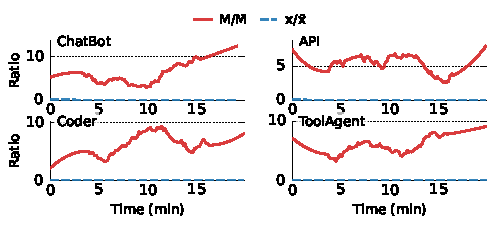
\includegraphics[width=0.98\linewidth ]{figs/5-3-detector/detector-allinone.pdf}
          \end{minipage} \\[1pt]
          \begin{minipage}{1\linewidth}
          \caption{\small{%
Empirical observations of the factors in the multiplicative score across different traces.
If $\frac{x}{\bar{x}} \leq \frac{|M|}{|\overline{M}|}$, no {\kvcache} hotspot can cause load imbalance,
so our multiplication method can effectively balance the load with {\kvcache}-awareness.
          }}  
          \label{fig:detector}
          \end{minipage} \\[-0pt]
          \end{figure}

\begin{equation}
\frac{x}{\bar{x}}
\leq
\frac{|M|}{|\overline{M}|}
\label{eq:consensus-1}
\end{equation}


{\fig{fig:detector}} shows that all traces---representative of LLM serving and studied in this work---are
benign to our method, because the expected batch size of the suspected hotspot instances is not larger than that of the others.
This can be interpreted as follows. 
Based on {\fig{fig:detector}}, we have the following observation summarized in Equation~\ref{eq:consensus-1} for all traces. 

\begin{equation}
\frac{x}{|M|}
\leq
\frac{\bar{x}}{|\overline{M}|}
\label{eq:consensus-2}
\end{equation}

\noindent
By rearranging the equation, we obtain Equation~\ref{eq:consensus-2}. 
Substituting into Equation~\ref{eq:bs-ratio-exact},
we get the expected batch size of the {\kvcache} hotspot instances is smaller than the others. 

\iffalse
As shown in \fig{fig:detector}, most observed classes satisfy
\(\frac{x}{\bar{x}} \leq \frac{|M|}{|\overline{M}|}\), indicating that benign
cases are common in practice and failure-prone patterns are uncommon.
\fi

\iffalse
\begin{equation}
  \frac{x}{\bar{x}} > \frac{|M|}{|\overline{M}|}.
  \label{eq:hotspot-condition}
\end{equation}
\fi

\stitle{Analysis: the failure cases, and our two-phase detector.  \,} 
Based on our previous analysis, we can see that if Equation~\ref{eq:consensus-1} 
does not hold, i.e., \[ \frac{x}{\bar{x}} > \frac{|M|}{|\overline{M}|}  \], 
then there is a potential for {\kvcache} hotspots to cause load imbalance
that may break our multiplication method. 
This gives a clear indication of the failure cases detector based purely on the workload pattern and {\kvcache} states, 
so we can develop a detector before we make a scheduling decision to catch potential failure cases. 

Specifically, for each request class, we profile the two terms \(\frac{x}{\bar{x}}\) and \(\frac{|M|}{|\overline{M}|}\) in real time,
and if we observe that Equation~\ref{eq:consensus-1} does not hold,
we raise an alarm and filter out the suspected instances (\(M\)) from the routing targets.
To avoid the overhead of tracking too many request classes, we only track the requests with the highest {\kvcache} hit rates.

One problem of the single-phase detector described above is that
even if Equation~\ref{eq:consensus-1} does not hold,
it may still be beneficial to route requests to the suspected instances with high {\kvcache} hit rates,
as long as we do not route too many requests to the hotspots.
Therefore, we further augment the detector with a second phase
by delaying the filtering until a consecutive number of requests are routed to hotspots,
as consecutive routing decisions may imply that the increase in the batch size of the suspected instances cannot offset the high {\kvcache} hit rates.

\begin{equation}
  \text{P-token}_m \times BS_m \leq \text{P-token}_{\bar{m}} \times BS_{\bar{m}}
  \label{eq:m-score}
\end{equation}

Specifically, after the first phase raises an alarm, we further track the new prefill tokens of the requests in this class,
and if we observe that more than \(2 \times M\) consecutive requests in the class have a smaller multiplicative score (Equation~\ref{eq:m-score}) on a suspected hotspot instance ($m$)
than on the rest of the instances ($\bar{m}$),
then we raise a second alarm that filters out the suspected instances from the routing targets.

\iffalse
Fortunately, we can use some relaxations to enable a more precise failure detector based on Equation~\ref{eq:bs-ratio-exact}.
More specifically, we can route requests to the suspected hotspot instances as long as 
\fi

\iffalse
%\stitle{Two-phase detector for the failure cases. \,}
We can compute \(\frac{x}{\bar{x}}\) and \(\frac{|M|}{|\overline{M}|}\), and 
utilize Eq~\eqref{eq:hotspot-condition} to design a detector catching potential failure cases. 
Specifically, if we observe a class-\(c\) unsatisfied with Eq~\eqref{eq:hotspot-condition} (phase-1), 
we mark this class suspicous and further track the new prefill tokens of the requests in this class.
If we observe more than \(2 \times M\) consecutive requests in the class with the following condition:
\[
  \frac{\text{P-token}_i}{\text{P-token}_j}
  \;\leq\;
  \frac{BS_j}{BS_i},
\]

\noindent
then we raise an alarm (phase-2) that forces a load-balancing scheduling policy
without considering {\kvcache} hits for the requests in this class. 
The rationale for the two-phase design stems from the false positive alarms of phase-1 detector, 
which is focus on only the necessary condition, rather than a sufficient-and-necessary one. 
In our evaluated traces the phase-1 detector filters out the entire workload, as shown in \fig{fig:detector}, 
indicating that no failure cases occur in our evaluation. 
Interestingly, we do detect one failure case in
evaluating {\sys} with another production trace of {\company}.
In this case, a user continuously sends requests with 3.2\,K input length and
these requests have a 98\% {\kvcache} hit rate for over 30 minutes, which accounts for 20\%
of the request arrival rate within a small cluster.
\fi

\iffalse
A failure occurs precisely when the left-hand side is much larger than the
right-hand side: even though instance \(i\in M\) already has a larger
batch size (i.e., \(BS_i > BS_j\)), the advantage in
\(\text{P-token}\) is so large that the policy continues to route
class-\(c\) requests to \(M\) instead of shifting them to
\(\overline{M}\) for load balancing.
This situation can arise when the {\kvcache} hit rate on \(M\) is extremely
high, making \(\text{P-token}_i\) almost zero and causing the ratio
\(\text{P-token}_i / \text{P-token}_j\) to dominate
Eq.~(\ref{eq:product-ratio-condition}).

To prevent such a corner case, we have developed a Monte-Caro (MC) detector which identifies
whether there is a group of requests with high {\kvcache} hits on the same prefix by sampling requests from traffic. 
If there is some class-\(c\), the MC detector examines the popularity and prefix cache to calculate two terms in Eq.~(\ref{eq:bs-ratio-approx}), 
and then compare it with {\kvcache} hit rate. If Eq.~(\ref{{eq:product-ratio-condition}}) is satisfied, then the router uses simple backup policies 
to schedule requests out of \(M\). 

In our evaluation traces we rarely observe such cases; however in our production trace, the MC detector has a true positive alarm. 
On such a circumstance, an inner user of {\company} continuously sends requests with 3.2k input length and 98\% {\kvcache} hit for 30 minutes, which occupies 20\% 
of the QPS within a small cluster. Our MC detector avoids routing these requests to a small set of instances, and thus keeps load balance.  
\fi
